% \textbf{This section should not be more than 2 columns.}

% World demand for food is expected to double by the year 2050, primarily driven by upward social mobility and an increase in the world population~\cite{godfray2010food}.
% The additional problems of climate change, water shortage, and reduced agricultural land are making the problem of meeting this increased demand significantly difficult. 
% It is estimated that data-driven agriculture practices can help reduce losses and improve yields, increasing overall productivity of the farms by 67\% by 2050. 
% There have been very successful field trials which show that varying the water input across different places on the farm based on sensor measurements can increase farm productivity by as much as 45\% while reducing the water input by 35\%~\cite{almarshadi2011effects}.  Similar techniques have proved to be very beneficial to other farm inputs such as fertilizers and seeds~\cite{kim2009soil}. While there has been a lot of work by big R\&D companies such as Microsoft Research and many startups on developing smart agricultural applications for farmers, these efforts are highly focused and there is a lack of open-source frameworks that enable multiple precision agriculture applications.
% \fatima{Only commercial efforts are not enough, infact academic input from agricultural and engineering experts is needed to better research the optimal use of technology in precision agriculture. It is imperative for academic community to produce open source hardware/software testbeds around precision agriculture to promote academic research.}
Small, family-owned farms represent 88\% of the 2.1 million farms in the United States. Collectively they occupy 48\% of the total land area of farms (915 million acres) yet represent only 20\% of overall agricultural sales according to the 2012 Census of Agriculture in the United States \cite{USDANati49:online}. These disproportionately small crop yields are likely due to the challenges inherent in the management of the complex dynamics involved in growing food. While larger industrial farms can afford optimizations through mechanization and advanced analytics, these techniques have seen only limited adoption in small farms.

Given that these small farms are so important to our overall food production needs, there lies a significant opportunity in improving their efficiency. Precision agriculture may offer a partial solution to these challenges by 1) increasing access to crop and climate data which can greatly improve yields and 2) automating and optimizing labor intensive tasks such as the application of pesticides, herbicides, and fertilizers. This new data-driven approach towards farming has the potential to reduce the amount of chemicals needed to maximize growth while simultaneously reducing material costs and risks to human health.

\begin{figure}[t]
\centering
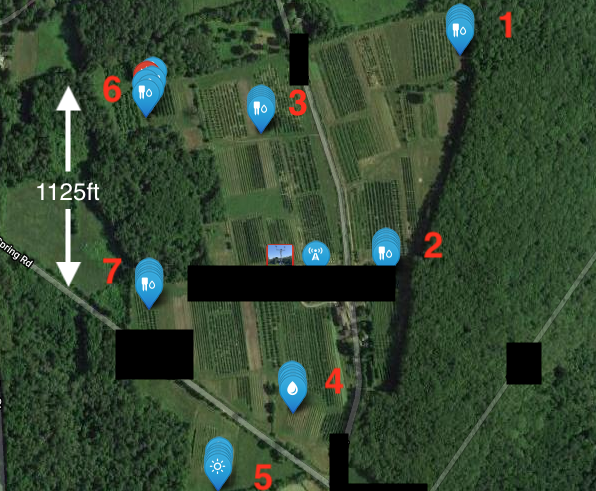
\includegraphics[width=0.3\textwidth]{./figures/orchardwatch.png}
% \vspace{-0.4cm}
\caption{Weather station deployment (Blinded for review)}
% \vspace{-0.3cm}
\label{fig:map}
\end{figure}

\begin{figure}[t]
\centering
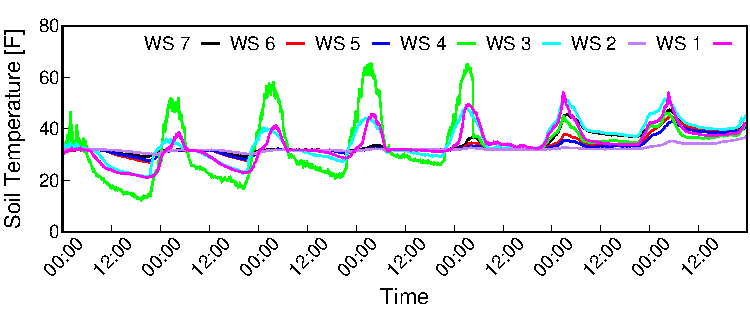
\includegraphics[width=0.42\textwidth]{./figures/soil_temp.pdf}
% \vspace{-0.4cm}
\caption{Soil temperature readings across seven weather stations (WS) over a one week period during Fall 2019.}
% \vspace{-0.3cm}
\label{fig:soil-temp}
\end{figure}

% \begin{figure}[t]
% \centering
% 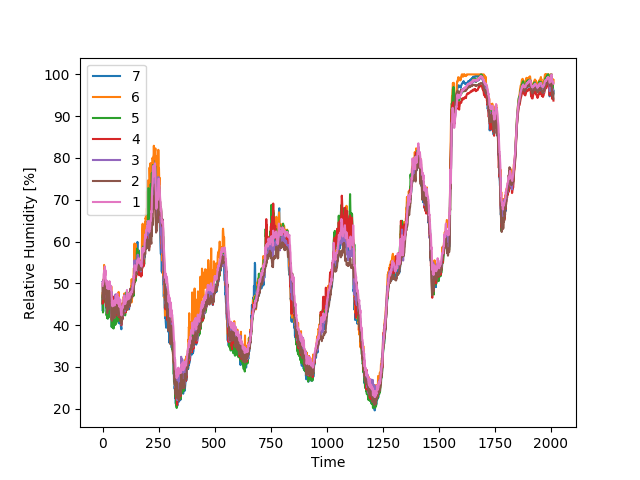
\includegraphics[width=0.4\textwidth]{./figures/relative_humidity.png}
% % \vspace{-0.4cm}
% \caption{Placeholder for Relative Humidity Figure}
% % \vspace{-0.3cm}
% \label{fig:relative-humidity}
% \end{figure}

In addition to increasing yields for small farms, agricultural researchers are another group that can benefit from this boom in precision agriculture through their experimentation at research farms. Agriculture researchers need more in-depth insights into farming systems, requiring visual and environmental data at a higher temporal and spatial resolution than what is needed by a traditional farmer~\cite{yield-prediction, crop-estimation, microclimate-specifics}. Current pest management and related crop production models are largely based on environmental data, particularly basic weather data such as temperature, rain and solar radiation~\cite{newa-model}. In almost all cases, this data comes from a single weather station on a farm, or if using virtual data, is at a resolution of 1 to 5 km. This ignores potentially important differences from one part of a farm to another, where microclimates may have different impacts on crops and pests~\cite{microcolimate-effect, microclimates, microclimate-specifics, microclimate-wsn}. To understand variations across microclimates, we deployed 7 networked weather stations at a research orchard near our campus at varying altitudes on a hillside (Figure~\ref{fig:map}). Figure~\ref{fig:soil-temp} shows that soil temperatures recordered by these weather stationscan vary by as much as $\sim$~20 degrees Fahrenheit across different locations. 
% \fatima{Its better to have references for all of these claims. What damage do micro climates and pests do etc. Ask Paul for these references} 

There is a need to gather environmental data at a much higher spatial and temporal resolution to support these research activities. Currently, pest management relies on individuals visiting fields and visually inspecting for the presence of insects, or for insect and disease damage, a process called scouting. This is critical in using environmentally sound pest management (pests include pathogens that cause disease), called integrated pest management (IPM)~\cite{ipm-greenhouse, ipm-overview}. The scouting process is generally performed every week, or at best every day, and involves a small portion of the entire crop~\cite{ipm-scouting}. An automated system that captures images frequently over a large portion of the crop, analyzes these images for relevant IPM information such as damage, and links the image to high-resolution environmental data, such as temperatures within individual plant canopies and would enable scientists to better understand the risk of pest damage. An appropriately simple interface would also enable growers to treat potential pest problems precisely when needed, and to treat only those plants at risk.

The field of precision agriculture is in its infancy, relative to the Internet-of-Things (IoT) and Wireless Sensor Networks (WSN). Precision agriculture shares many goals and constraints of IoT and WSN, such as resource-constrained devices, in-field deployments, and need for ubiquity. The research work on precision agriculture has borrowed heavily from prior work on WSN and IoT, as summarized by Thakur et al~\cite{thakur2019applicability}. FarmBeats is the most well-known IoT platform for data-driven agriculture~\cite{vasisht2017farmbeats, kapetanovic2017experiences, jain2019low} that shares high level goals of our project. The key drawback of FarmBeats is the lack of flexibility in the architecture, i.e. requiring the presence of a farmer's home at the farm with a computer and internet connectivity. These assumptions may not be true for many farms, especially in remote rural communities in the US and especially in developing countries. FarmBeats is primarily a data acquisition system and does not possess the capability to perform real-time inferences and control over actuators inside the farm, i.e. processing visual data in real-time to release pesticides. Finally, the system primarily provides soft sensor values that are interpolated from image maps that are linked to sparsely-deployed sensors -- unless the image maps are updated frequently, the overall system will achieve limited accuracy. 

% It shares the high level goals of our project for monitoring farm and having processing capabilities at the edge, but it is not scalable and does not allow the implementation of generic precision agriculture applications. 
% Our goal is to build an interactive, near real-time, and extensible framework that monitors the smallest component in the farm i.e. leaves as well as whole trees, so that the agriculture scientists can use this rich temporal and spatial data to understand the impact of micro-climates as well as enable different precision agriculture applications.


\myname, is a three-tiered edge computing architecture for precision agriculture applications that is \emph{simple}, \emph{extensible}, and \emph{open-source}. The primary goal of \myname{} is to simplify data access and application deployment for small farms and academic researchers that require innovative and practical precision agriculture applications, but are not IoT experts. 
%This approach differs from existing platforms, such as FarmBeats~\cite{vasisht2017farmbeats}, which require familiarity with embedded devices and Microsoft Azure to access and develop applications. Researchers and farmers may not have such expertise or time to learn and develop FarmBeats applications. 
\myname{} satisfies the constraint of developing a low-power and low cost solution: it runs on a solar panel with a battery backup and the core design components cost less than \$5000 for monitoring a 220ft by 30ft field of trees. 

% \myname's \emph{extensible} design is based on a vertically integrated three-tiered architecture. The bottom-tier consists of densely deployed battery-free backscatter sensors that provide high granularity data for environmental variables i.e. temperature, humidity, soil moisture; these devices are intermittently powered by readers or carrier emitters at the mid-tier. The mid-tier also comprises devices capable of capturing and processing high-resolution data such as high resolution images and video streams. The mid-tier is networked with actuators (i.e robotic spray units, camera steering, irrigation) to enable low latency closed-loop control. The top-tier is a cloud component connected to the mid-tier through an unreliable network at relatively high latency.

There are multiple challenges that need to be addressed at each layer. At the bottom tier, the distance of the devices from the reader and power source at the mid-tier needs to be carefully calibrated for optimal data collection. The duration and intensity of the power source to ensure an accurate reading from intermittently powered devices is also an open challenge. At the mid tier, managing bottom-tier nodes opens new research problems. In addition, it also needs to manage energy harvesting, forecasting energy into the future, and managing energy budget given data processing and inference needs. Finally, at the top tier, a carefully designed user interface is needed to ensure smooth user experience. The challenges and possible solutions at each layer are discussed in Section~\ref{design}. 



% The OrchardScope node allows easy integration of new sensors and facilitates deployment of ML applications at the edge. OrchardScope network is scalable and uses dedicated radios to enable node-node, node-cloud, and node-vehicle communication. OrchardScope application tier allows users to view and use data pipelines to build different applications. We plan to \emph{publicly release} OrchardScope as open-source to advance precision agriculture research and applications that require visual and environmental data at various resolutions with different response times. Our hypothesis is that this design can provide researchers and farmers a simple way to acquire high resolution data and enable the implementation of existing and new precision agriculture applications. 

% In this paper, we present OrchardScope, a network and computing architecture for precision agriculture, that seamlessly enables different applications with very different data requirements, computation needs, and allowing different times to react. OrchardScope can ensure system availability  even  in  the  face  of  power  and  Internet  outages caused by bad weather, a fairly common scenario for a farm.  Further, OrchardScope enables cloud connectivity for the sensor data for user access and to enable persistent storage as well as long-term or cross-farm analytics. We plan to deploy our system on a green house managed by a research university as well as a research orchard managed by the agriculture department of a major public university in United States. At the start, we plan to enable three applications for the researchers: monitoring experiments in the greenhouse, automating apple cluster thinning task for apple orchard, and gathering large-scale visual data for disease detection. In designing OrchardScope, we solve three key challenges. 

% First, to enable gathering of high resolution visual and environmental data, we design a mesh network of resourceful devices called OrchardScope nodes that are spread throughout the farm. The camera and other sensors directly connect with the node. There is a lack of power on the farm and these devices are powered by the solar panels with a battery backup. As solar power is impacted by the weather significantly, there has been some work on developing weather-aware edge devices that modulate their operations based on the weather forecasts~\cite{vasisht2017farmbeats}. However, the prior work uses outdated and inaccurate forecasting techniques. We plan to leverage recent work on developing probabilistic weather forecasts that give a distribution solar power based on the weather forecast. The probabilistic forecast approach help understand the uncertainty in the forecast value and accounting that in the operation of the OrchardScope node helps make the system more reliable. 

% Second,  Internet  connection  to  the  farm  is  typically weak or in some cases non-existent making it challenging to ship high bandwidth visual data collected from the OrchardScope nodes to the cloud for processing. 
% To counter this problem, we design our system with an assumption that there is no Internet connectivity to the farm in the form of high-speed internet connection from Internet providers. This constraint pushes our design towards edge computing where we equip the OrchardScope nodes with the embedded devices capable of running computer vision and machine learning tasks. We also enable collaborative edge computing for the cases where a single device will not be able to satisfy the processing needs of a particular application. We send high level summaries and data to the cloud where the researchers and farmers can get access to the data. We are also considering providing access to the data within the farm, if needed. 

% Finally, while drones are one of the most exciting farm sensors today, they suffer from poor battery life. Getting aerial imagery for a farm requires multiple drone flights and a long wait time in between when the batteries are being charged. These characteristics are not suitable for our intended applications where we may need data of various parts of a single tree every few minutes, i.e. capturing multiple apple clusters on a single tree every 20 minutes. Therefore, we decide on the static placement of cameras inside the farm where each camera captures multiple trees and provides high resolution images of very tiny parts of the trees.\fatima{I think we should not highlight static placement because we have the capability of rotation and zooming in on a particular event of interest.} Our cameras use computer vision and image processing techniques to enable capturing of very small parts of the tree or get wide views that may be needed for some applications. 



% \fatima{Comment on the cost of your test bed.}

% % The rest of the paper is organized as follows. We describe the high level architecture of the OrchardScope in Section~\ref{fig:architecture}. The design details for the OrchardScope node are given in Section~\ref{node}, while the network details are outlined in Section~\ref{network}. The application tier is described in the Section~\ref{application}. Finally, we will present our deployment details in Section~\ref{deployments}. 
% % % \fatima{We can remove this paragraph.}

% \fatima{It's good to write it in context of an architecture that caters to various precision agriculture applications and is extensible in terms of it's sensing, network, and compute capability to support future applications}